\documentclass{hw}

\usepackage{amssymb} %% Latex特殊符号对应表  见https://blog.csdn.net/caiandyong/article/details/53351737
\usepackage {indentfirst}  %% 中文首行缩进,需要首行缩进的段落前加上代码“\setlength{\parindent}{2em}”即可
%% 不想首行缩进, 在段落前使用命令 \noindent
\usepackage{cite}
\usepackage{natbib}   %% 引用格式问题
\setcitestyle{numbers,compress,square,comma,super}
%\usepackage[sectionbib]{chapterbib} %% 分章节参考文献
\usepackage[hyperfootnotes=false]{hyperref}
\hypersetup{
  colorlinks,
  citecolor=red,
  linkcolor=blue,
  urlcolor=blue,
 % citebordercolor=Violet,
 % filebordercolor=Red,
 % linkbordercolor=Blue
}
\usepackage{color} %% 批注颜色设置 \color{blue}这一排的字体是蓝色。 或者 \textcolor[rgb]{1,0,0}{text}
\usepackage[d]{esvect} %% 矢量箭头 见https://mirrors.bfsu.edu.cn/CTAN/macros/latex/contrib/esvect/esvect.pdf
\usepackage{tabularray} %% 表格的使用(P46有关于diagbox的说明)https://mirrors.ustc.edu.cn/CTAN/macros/latex/contrib/tabularray/tabularray.pdf 非常Nice
\UseTblrLibrary{diagbox}
\UseTblrLibrary{booktabs}
%% 嵌入MATLAB代码块 见https://mirrors.ustc.edu.cn/CTAN/macros/latex/contrib/matlab-prettifier/matlab-prettifier.pdf,也可参考以下https://zhuanlan.zhihu.com/p/388676497
\usepackage{listings}
\usepackage{xcolor}
\usepackage{textcomp}
\usepackage{matlab-prettifier}
%% 使用时只需要添加以下代码即可:\lstinputlisting[style=Matlab-editor,basicstyle=\mlttfamily,numbers=left,frame=single,caption={\bf main.m}]{L3/sample.m}
\usepackage{graphicx}
\usepackage{ragged2e} %% 首行缩进
\usepackage{float} %% 图片位置固定
%% 关键信息高亮 见https://latex-tutorial.com/color-latex/
\usepackage[dvipsnames]{xcolor}
\usepackage{soul}
\usepackage{xcolor}
%% 斜分数 \nicefrac{}{}
\usepackage{units}

\course
{纳米光子学及其应用}
{Fall 2022}
{UESTC}

\assignment
{第一次作业}
{11个思考题}

\student
{张豪}
{202221050516}
{Z\_Howe94@163.com}

\begin{document}
%\sethlcolor {Aquamarine} %% 高亮颜色 使用方式:\hl{Englishtext} 或 \hl{\mbox{中文text}}

\newproblemset{problem}{思考}{思考题}
\newproblemset{computerexercise}{Computer Exercise}{Computer Exercises}
\newcommand{\pll}{\kern 0.56em/\kern -0.8em /\kern 0.56em}
\maketitle

\makeproblem

\begin{problem} % 1
为什么物体的维度小于电子的德布罗意波长,量子效应就显著?
\end{problem}

\begin{answer*}

%\justifying{\setlength{\parindent}{2em}{当物体的尺寸小到可与电子的徳布罗意波长,相干波长及激子波尔半径相比时,电子的局限性和相干性增强,极易形成激子,产生激子吸收带。随着粒径的进一步减小,激子带的吸收系数增加,出现激子强吸收。由于量子约束效应,激子的最低能量向高能方向移动,其光谱是由带间跃迁的一系列谱线组成的。载流子运动受到限制,费米能级附近的电子能级由准连续变成分立,即能量发生量子化。量子尺寸效应导致其吸收谱从连续分布,变为具有峰值结构的离散谱带。}

\justifying{\setlength{\parindent}{2em}{我们不妨考虑物体的尺寸为$L_z$,电子在无限深的势阱内运动(势阱两边是物体边缘),相应的电子波函数$\psi(z)$满足薛定谔方程:}
\[
-\dfrac{\hbar^2}{2m}\dfrac{d^2}{dz^2}\psi(z)+U(z)\psi(z)=E\psi(z)
\]

\justifying{\setlength{\parindent}{2em}{$E$为电子沿$z$方向运动的能量,而限制电子运动的势能函数$U(z)$可以表示为}
\begin{equation}
	U(z) =
	\begin{cases}
		0, & (-L_z/2<z<L_z/2) \\
		\infty, & (z<-L_z/2,z>L_z/2)}
	\end{cases}
	\label{eq11}
\end{equation}

\justifying{\setlength{\parindent}{0em}{由于势垒无限高,电子不能逸出势阱,即在$z=\pm L_z/2$处波函数$\psi(z)$必须是0。利用这一条件可以得出,电子沿$z$方向运动的能量只能取下述的分立值:}
\[
E_{nc}=\dfrac{(\pi\hbar)^2}{2m_e^*}(\dfrac{n}{L_z})^2 \qquad n=1,2,3,\cdots
\]

\justifying{\setlength{\parindent}{0em}{相应的波函数为}
\begin{equation}
	\psi_n(z) =
	\begin{cases}
		\cos (n\dfrac{\pi}{L_z}z), & n=1,3,5,\cdots \vspace{1em} \\
		\sin (n\dfrac{\pi}{L_z}z), & n=2,4,6,\cdots
	\end{cases}
	\label{eq12}
\end{equation}

\justifying{\setlength{\parindent}{0em}{另一方面,电子在$x-y$平面内自由运动,能量连续变化,}
\[
E_{xy}=\dfrac{\hbar^2}{2m_e^*}(k_x^2+k_y^2)=\dfrac{\hbar^2k_\perp^2}{2m_e^*}
\]

\justifying{\setlength{\parindent}{0em}{$k_x$和$k_y$分别为$x$方向和$y$方向的电子波矢。所以,电子在势阱中运动的总能量为}
\[
E_c(k\prep,n)=\dfrac{\hbar^2k_\perp^2}{2m_e^*}+\dfrac{(\pi\hbar)^2}{2m_e^*}(\dfrac{n}{L_z})^2 \qquad n=1,2,3,\cdots
\]

\justifying{\setlength{\parindent}{2em}{不妨取$n=1$和$n=2$,其能量间隔为:}
\[
\Delta E=\dfrac{(\pi\hbar)^2}{2m_e^*}(\dfrac{2}{L_z})^2-\dfrac{(\pi\hbar)^2}{2m_e^*}(\dfrac{1}{L_z})^2=\dfrac{(\pi\hbar)^2}{2m_e^*}\dfrac{3}{L_z^2}
\]
\justifying{\setlength{\parindent}{0em}{对于电子的德布罗意波长满足下式:}
\[
\dfrac{1}{2m_e^*}=\dfrac{\lambda_e^2}{h^2}k_BT
\]
\justifying{\setlength{\parindent}{0em}{代入能量间隔表达式,可以简化为:}
\[
\Delta E=\dfrac{3}{4}(\dfrac{\lambda_e}{L_z})^2k_BT
\]
\justifying{\setlength{\parindent}{0em}{由上式可以看出,相邻能级之间的能量间隔与$k_BT$有关。当物体尺寸$L_z\gg\lambda_e$时,能级间距越来越小,可以看做连续能级,此时给予电子一定的热激发,电子几乎可以在各个能级之间运动,那么也就不能有“能级”一说了;而当物体尺寸与电子的德布罗意波长相当或者$L_z\ll\lambda_e$时,能级间距越来越大($>k_BT$),可以看做离散能级,此时,只有输入能量$\sim k_BT$时才能激发电子进行能级跃迁,即量子效应愈发显著。}
\end{answer*}

\begin{problem} % 2
对于半导体纳米晶,什么是弱限制,什么是强限制? 强、弱限制情况下对应体系能量如何表示? 哪一种限制可以使半导体量子点的光吸收边大于带隙宽度?
\end{problem}

\begin{answer*}

\justifying{\setlength{\parindent}{2em}{对于具有无限电势的球形势场以及具有各向同性有效质量的电子和空穴,可以针对两种极限情况得出强限制和弱限制的体系能量。}


\fcolorbox{white}{green}{\mbox{1、弱限制}}

\justifying{\setlength{\parindent}{2em}{假定我们的纳米晶为球形,其半径为$a$,且满足$a\gg a_B^{*}$时,其中$a_B^{*}$为激子玻尔半径。这种情况我们称之为弱限制。此时,激子的能量可以表示为:}
\[
E_{nml}=E_g-\dfrac{\text{Ry}^*}{n^2}+\dfrac{\hbar^2\chi_{ml}^2}{2Ma^2},\qquad n,m,l=1,2,3,...	
\]

\justifying{\setlength{\parindent}{2em}{其中,$\chi_{ml}$为贝塞尔函数的根,如表1所示。$M=m_e^*+m_h^*$为激子质量,等于电子有效质量$m_e^*$和空穴有效质量$m_h^*$之和。}
\begin{table}[H]
    \centering
    \fontsize{8}{10}\selectfont    %{字体尺寸}{行距}
    \caption{贝塞尔函数$\chi_{nl}$的根}
	\begin{tblr}{
        row{odd} = {bg=azure8},
        row{1} = {bg=azure3, fg=white},
        colspec={c|ccc},
        }
	    \toprule
		$l$ & $n=1$ & $n=2$ & $n=3$ \\
	    \specialrule{0.5pt}{4pt}{6pt}
		0 & 3.142(\pi) & 6.283(2\pi) & 9.425(3\pi)\\
        1 & 4.493 & 7.725 & 10.904\\
        2 & 5.764 & 9.095 & 12.323\\
        3 & 6.988 & 10.417 &  \\
        4 & 8.183 & 11.705 &  \\
        5 & 9.356 &   &  \\
        6 & 10.513 &   &  \\
        7 & 11.657 &   &  \\
	    \bottomrule 
	\end{tblr}
   % \label{tab:1}
\end{table}

\fcolorbox{white}{green}{\mbox{2、强限制}}

\justifying{\setlength{\parindent}{2em}{假定我们的纳米晶为球形,其半径为$a$,且满足$a\ll a_B^{*}$时,其中$a_B^{*}$为激子玻尔半径。这种情况我们称之为强限制。此时,对于最低能级$1s1s$态,激子能量可以表示为:}
\[
E_{\text{1s1s}}=E_g+\pi^2(\dfrac{a_B^*}{a})^2\text{Ry}^*-1.786\dfrac{a_B^*}{a}\text{Ry}^*-0.248\text{Ry}^*	
\]

\justifying{\setlength{\parindent}{2em}{强限制可以使半导体量子点的光吸收边大于带隙宽度,对于理想量子点而言(如下图所示),强限制使得原本连续的吸收谱(吸收峰在禁带)离散化,此时的多个吸收峰均高于禁带。}

\begin{figure}[H]
\centering
	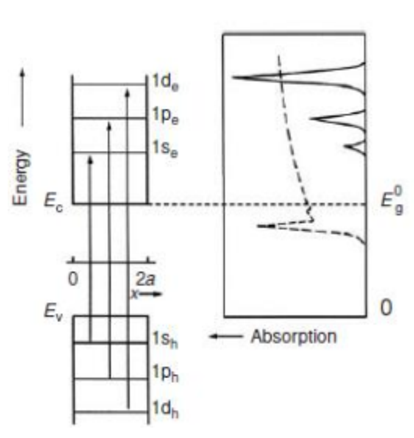
\includegraphics[width=0.4\textwidth]{L3/f9.pdf}
\caption{\justifying{理想量子点能级与吸收谱}}
\label{f10}
\end{figure}

\end{answer*}

\begin{problem} % 3
为什么不能用空间光直接激发体积等离子体振荡?
\end{problem}

\begin{answer*}

\justifying{\setlength{\parindent}{2em}{在外场$E(t)=E_0\text{exp}(-i\omega t)$作用下,金属中的自由电子可以看成是没有回复力的谐振子,此时自由电子的运动方程可以写成:}
\begin{equation}
m\ddot{\boldsymbol{r}}+m\gamma\dot{\boldsymbol{r}}=-e\boldsymbol{E}
\label{eq:a3}
\end{equation}

\justifying{\setlength{\parindent}{2em}{式(\ref{eq:a3})中的$\gamma$为阻尼频率。通过求解该运动方程,可以求出金属的介电常数为:}
\begin{equation}
\epsilon(\omega)=1-\dfrac{\omega_p^2}{\omega^2+i\omega\gamma},\qquad \omega_p=\sqrt{\dfrac{Ne^2}{\varepsilon_0m}}
\label{eq:4}
\end{equation}
\justifying{\setlength{\parindent}{2em}{其中,$\omega_p$为体积等离子体激元的固有频率。}

\justifying{\setlength{\parindent}{2em}{对于空间光而言,有$\gamma\ll\omega<\omega_p$,此时由于$\omega\gg\gamma$,故金属的介电常数可以简化为:}
\[
\varepsilon(\omega)\approx1-\dfrac{\omega_p^2}{\omega^2}
\]
此时,$\varepsilon<0$,故对应的金属折射率$n$是一个复数,可以表示为$n=\sqrt{\varepsilon}=n'+in''$。根据以上两式可以求得:
\[
n'=0,\qquad n''=\sqrt{\dfrac{\omega_p^2}{\omega^2}-1}
\]

由之前运动方程求解得到的金属中的电场可以写成以下形式:
\[
\boldsymbol{E}=\boldsymbol{E}_0\text{exp}(i\boldsymbol{k}\cdot\boldsymbol{r})=\boldsymbol{E}_0\text{exp}(in\boldsymbol{k}_0\cdot\boldsymbol{r})=\boldsymbol{E}_0\textcolor[rgb]{1,0,0}{\text{exp}(-n''\boldsymbol{k}_0\cdot\boldsymbol{r})}
\]
可以看到,金属中的电场存在\textcolor[rgb]{1,0,0}{衰减项},即金属中的场呈现指数衰减,因此不能用空间光直接激发体积等离子体振荡。

\end{answer*}

\begin{problem} % 4
体积等离子体频率的物理意义是什么?
\end{problem}

\begin{answer*}

当入射波频率$\omega=\omega_p$,即处于等离子体频率时,金属介电常数$\varepsilon$约为$0$(考虑$\omega\gg\gamma$的情况)。通过下式的波动方程可以得到:
\[
\boldsymbol{k}(\boldsymbol{k}\cdot\boldsymbol{E})-\boldsymbol{k}^2\boldsymbol{E}=-\varepsilon\dfrac{\omega^2}{c^2}\boldsymbol{E}
\]
只有当金属中的$\boldsymbol{k}\pll\boldsymbol{E}$,才能满足$\varepsilon\approx 0$。说明此时只有自由电子的\textcolor[rgb]{1,0,0}{集体纵向振荡}存在,\textcolor[rgb]{1,0,0}{这不是一个传导波}。且由于此时的波为纵波,故它不与横向电磁波发生作用,二者波矢无法匹配。

需要注意的是,由于$\boldsymbol{k}\pll\boldsymbol{E}$,因此根据Maxwell方程组中的:
\[
\nabla\times\boldsymbol{E}=-\dfrac{\partial\boldsymbol{B}}{\partial t}\Rightarrow\boldsymbol{k}\times\boldsymbol{E}=\omega\mu \boldsymbol{H}
\]
得到$\boldsymbol{H}=0$,即不存在$\boldsymbol{E}$和$\boldsymbol{H}$的相互作用。
\end{answer*}

\begin{problem} % 5
试结合Maxwell方程组和界面边界条件推导SPP的色散关系。
\end{problem}

\begin{answer*}

当\textcolor[rgb]{1,0,0}{电流密度$\boldsymbol{J}_{\text{ext}}$为0}时,将本构关系代入Maxwell方程组中的法拉第定律和安培-麦克斯韦定律中,可得:
\[
(\textcolor[rgb]{1,0,0}{1})\text{法拉第定律:} \nabla\times\boldsymbol{E}=-\dfrac{\partial\boldsymbol{B}}{\partial t}
\]\[
(\textcolor[rgb]{0,0,1}{2})\text{安培-麦克斯韦定律:} \nabla\times\boldsymbol{B}=\mu_0\varepsilon_0\varepsilon\dfrac{\partial\boldsymbol{E}}{\partial t}
\]
对$(\textcolor[rgb]{1,0,0}{1})$式取旋度,可以得到:
\[
\nabla\times\nabla\times\boldsymbol{E}=-\dfrac{\partial}{\partial t}\nabla\times\boldsymbol{B}
\]
将$(\textcolor[rgb]{0,0,1}{2})$式代入上式,可以得到:
\[
\nabla\times\nabla\times\boldsymbol{E}=-\mu_0\varepsilon_0\varepsilon\dfrac{\partial^2\boldsymbol{E}}{\partial t^2}
\]
根据\fcolorbox{red}{white}{$\nabla\times\nabla\times\boldsymbol{E}=\nabla(\nabla\cdot\boldsymbol{E})-\nabla^2\boldsymbol{E}$}可将上式化简为:
\[
\nabla(-\dfrac{1}{\varepsilon(\boldsymbol{r})}\boldsymbol{E}\cdot\nabla\varepsilon)-\nabla^2\boldsymbol{E}+\dfrac{\varepsilon}{c^2}\dfrac{\partial^2\boldsymbol{E}}{\partial t^2}=0
\]
我们假定\fcolorbox{red}{white}{$\varepsilon(\boldsymbol{r})=\varepsilon$},即与位置无关,则上式可进一步简化为:
\[
\nabla^2\boldsymbol{E}-\dfrac{\varepsilon}{c^2}\dfrac{\partial^2\boldsymbol{E}}{\partial t^2}=0
\]
考虑到时谐电场可写为\fcolorbox{red}{white}{$\boldsymbol{E}=\boldsymbol{E}(x,y,z)\text{exp}(-i\omega t)$},且真空中光波波矢为$k_0=\omega/c$,可以得到电场所满足的亥姆霍兹方程表达式:
\[
\nabla^2\boldsymbol{E}+k_0^2\varepsilon\boldsymbol{E}=0
\]
在分析表面等离子体时,我们希望通过边界条件求解Maxwell方程组得到的解应当满足:在两个材料界面的电磁波沿$x$方向传播,且沿$z$方向呈指数衰减形式分布,如图\ref{f1}所示。
\begin{figure}[H]
\centering
	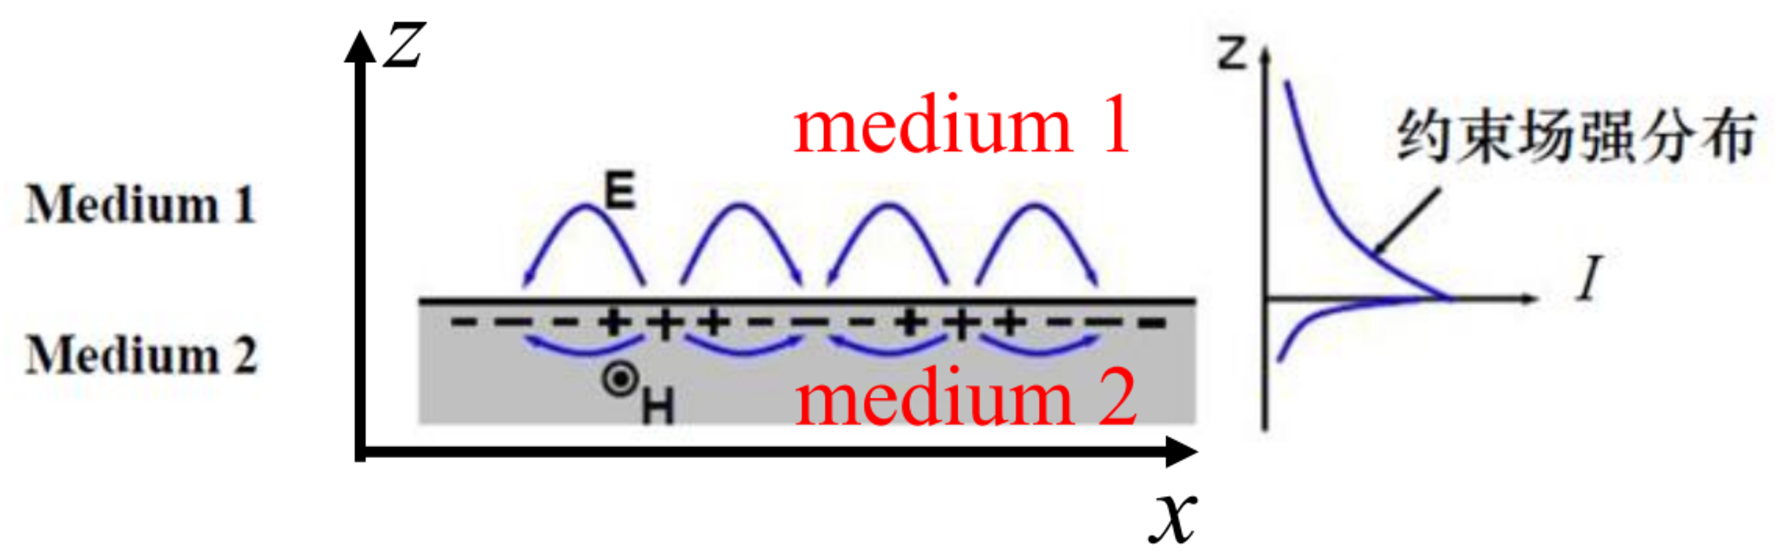
\includegraphics[width=0.7\textwidth]{L3/f1.pdf}
\caption{\justifying{SPP的场分布}}
\label{f1}
\end{figure}
\justifying{\setlength{\parindent}{2em}{因此,我们令\fcolorbox{red}{white}{$\boldsymbol{E}(x,y,z)=\boldsymbol{E}(z)\text{exp}(i\beta x),\beta=k_x$},其中$\beta$为传播常数,即$x$方向的波数$k_x$,代入亥姆霍兹方程,可得:}
\[
\dfrac{\partial^2\boldsymbol{E}(z)}{\partial z^2}+(k_0^2\varepsilon-\beta^2)\boldsymbol{E}(x,y,z)=0
\]

\justifying{\setlength{\parindent}{0em}{由于SPP波要在$z$方向衰减,因此需满足\fcolorbox{red}{white}{$k_0^2\varepsilon-\beta^2<0$},令$(ik_z)^2=k_0^2\varepsilon-\beta^2$,即$k_z^2-\beta^2+k_0^2\varepsilon=0$,此时方程化为了:}
\[
\dfrac{\partial^2\boldsymbol{E}}{\partial z^2}-k_z^2\boldsymbol{E}=0
\]
其解为:$\boldsymbol{E}=\boldsymbol{E}_0\text{exp}(\pm k_zz)$。

\justifying{\setlength{\parindent}{2em}{综上,根据求解Maxwell方程,我们得到了电磁波沿$x$方向传播,场量与$y$无关,且在$z=0$两侧衰减的电磁场基本表达式为:}
\[
\boldsymbol{E}(x,z)=\boldsymbol{A_1}e^{\pm k_zz}e^{i\beta x}e^{-i\omega t}
\]
\[
\boldsymbol{H}(x,z)=\boldsymbol{A_2}e^{\pm k_zz}e^{i\beta x}e^{-i\omega t}
\]
这里需要注意的是,$k_z$本身大于0,正负号的选择取决于介质层,若$z>0$,则取$(-)$号;若$z<0$,则取$(+)$号。

\justifying{\setlength{\parindent}{2em}{知道SPP的电磁场分布基本解后,我们需要根据边界条件求SPP的色散关系。同样地,假设电流密度$\boldsymbol{J}_{\text{ext}}$为0,将本构关系$\boldsymbol{H}=\boldsymbol{B}/\mu_0$和$\nicefrac{\partial}{\partial t}=-i\omega$代入Maxwell方程组中的法拉第定律和安培-麦克斯韦定律中,可得:}
\begin{align*}
(1)\left\{
\begin{array}{l}  
  \dfrac{\partial E_z}{\partial y}-\dfrac{\partial E_y}{\partial z}=i\omega\mu_0H_x \vspace{1ex} \\ 
  \dfrac{\partial E_x}{\partial z}-\dfrac{\partial E_z}{\partial x}=i\omega\mu_0H_y \vspace{1ex} \\
  \dfrac{\partial E_y}{\partial x}-\dfrac{\partial E_x}{\partial y}=i\omega\mu_0H_z 
\end{array} 
\right.
(2)\left\{
\begin{array}{l}  
  \dfrac{\partial H_z}{\partial y}-\dfrac{\partial H_y}{\partial z}=i\omega\varepsilon_0\varepsilon E_x \vspace{1ex} \\ 
  \dfrac{\partial H_x}{\partial z}-\dfrac{\partial H_z}{\partial x}=i\omega\varepsilon_0\varepsilon E_y \vspace{1ex}\\
  \dfrac{\partial H_y}{\partial x}-\dfrac{\partial H_x}{\partial y}=i\omega\varepsilon_0\varepsilon E_z 
\end{array} 
\right.
\end{align*}
将\fcolorbox{red}{white}{$\dfrac{\partial}{\partial x}=i\beta$、$\dfrac{\partial}{\partial y}=0$、$\dfrac{\partial}{\partial z}=\pm k_z$}代入上式,可得:
\begin{align*}
(1)\left\{
\begin{array}{l}  
  \textcolor[rgb]{1,0,0}{\pm k_zE_y=-i\omega\mu_0H_x} \vspace{1ex} \\ 
  \textcolor[rgb]{0,0,1}{\pm k_zE_x-i\beta E_z=i\omega\mu_0H_y} \vspace{1ex}\\
  \textcolor[rgb]{1,0,0}{i\beta E_y=i\omega\mu_0H_z}
\end{array} 
\right.
(2)\left\{
\begin{array}{l}  
  \textcolor[rgb]{0,0,1}{\pm k_zH_y=i\omega\varepsilon_0\varepsilon E_x} \vspace{1ex} \\ 
  \textcolor[rgb]{1,0,0}{\pm k_zH_x-i\beta H_z=-i\omega\varepsilon_0\varepsilon E_y} \vspace{1ex}\\
  \textcolor[rgb]{0,0,1}{i\beta H_y=-i\omega\varepsilon_0\varepsilon E_z}
\end{array} 
\right.
\end{align*}
\justifying{\setlength{\parindent}{2em}{从上式可以看到,这六个等式可以分为两套独立的解,分别为:}
\begin{align*}
(\textcolor[rgb]{0,0,1}{1})\left\{
\begin{array}{l}  
  \textcolor[rgb]{0,0,1}{E_x=\pm k_zH_y/i\omega\varepsilon_0\varepsilon} \vspace{1ex}\\
  \textcolor[rgb]{0,0,1}{E_z=-\beta H_y/\omega\varepsilon_0\varepsilon} \vspace{1ex} \\ 
  \textcolor[rgb]{0,0,1}{(k_z^2-\beta^2+k_0^2\varepsilon)H_y=0}
\end{array} 
\right.
(\textcolor[rgb]{1,0,0}{2})\left\{
\begin{array}{l}  
  \textcolor[rgb]{1,0,0}{H_z=\beta E_y/\omega\mu_0} \vspace{1ex} \\
  \textcolor[rgb]{1,0,0}{H_x=\pm k_zE_y/(-i\omega\mu_0)} \vspace{1ex} \\
  \textcolor[rgb]{1,0,0}{(k_z^2-\beta^2+k_0^2\varepsilon)E_y=0} 
\end{array} 
\right.
\end{align*}
这两套解分别对应着两种模式,即TM模和TE模,如图\ref{f2}所示。
\begin{figure}[H]
\centering
	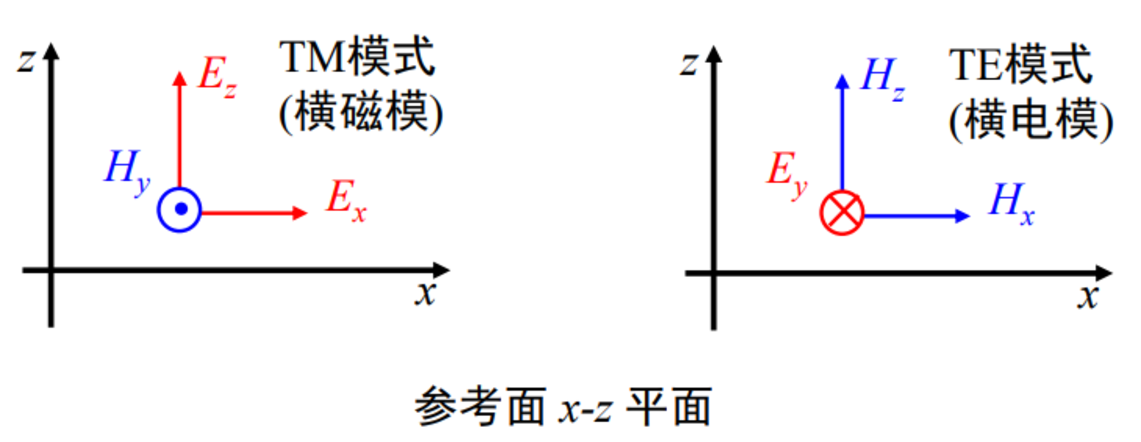
\includegraphics[width=0.7\textwidth]{L3/f2.pdf}
\caption{\justifying{两套独立解分别代表着TM模和TE模}}
\label{f2}
\end{figure}

\justifying{\setlength{\parindent}{2em}{先考虑TM波的情况:由于在介质1和介质2的分界面有\fcolorbox{red}{white}{$H_y$和$E_x$切向连续}这一边界条件,故对\textcolor[rgb]{0,0,1}{$\pm k_zH_y=i\omega\varepsilon_0\varepsilon E_x$}运用边界条件,可得:}
\begin{align*}
\left\{
\begin{array}{l}  
  -k_{z1}H_{y1}=i\omega\varepsilon_0\varepsilon_1E_{x1} \text{(in Medium 1)}\vspace{1ex}\\
  k_{z2}H_{y2}=i\omega\varepsilon_0\varepsilon_2E_{x2} \text{(in Medium 2)}
\end{array} 
\right.
\end{align*}
对以上两式做比值,得到:
\[
\dfrac{k_{z1}}{k_{z2}}\cdot\dfrac{H_{y1}}{H_{y2}}=-\dfrac{\varepsilon_1}{\varepsilon_2}\cdot\dfrac{E_{x1}}{E_{x2}}
\]
化简得:
\[
\dfrac{k_{z1}}{k_{z2}}=-\dfrac{\varepsilon_1}{\varepsilon_2}
\]
若要保证$k_{z1}$和$k_{z2}$均大于零,则$\varepsilon_1$和$\varepsilon_2$必须异号,即两介质应为金属和电介质。

\justifying{\setlength{\parindent}{2em}{由于$k_z^2=\beta^2-k_0^2\varepsilon$,故在不同的介质中有不同的表达式:}
\begin{align*}
\left\{
\begin{array}{l}  
  k_{z1}^2= \beta^2-k_0^2\varepsilon_1 \text{(in Medium 1)}\vspace{1ex}\\
  k_{z2}^2= \beta^2-k_0^2\varepsilon_2 \text{(in Medium 2)}
\end{array}   
\right.
\end{align*}
联立该式($\dfrac{k_{z1}}{k_{z2}}=-\dfrac{\varepsilon_1}{\varepsilon_2}$),可以得到SPP的色散关系为:
\[
\beta=k_0\sqrt{\dfrac{\varepsilon_1\varepsilon_2}{\varepsilon_1+\varepsilon_2}}=\dfrac{\omega}{c}\sqrt{\dfrac{\varepsilon_m\varepsilon_d}{\varepsilon_m+\varepsilon_d}}
\]
\end{answer*}

\begin{problem} % 6
为什么不存在TE模式的位于金属-介质界面的表面波?试结合Maxwell方程组和边界条件进行分析。
\end{problem}

\begin{answer*}

\justifying{\setlength{\parindent}{2em}{同“思考题5”一样,根据SPP的电磁场分布基本解求解Maxwell方程组得到两组独立的解,即:}
\begin{align*}
(\textcolor[rgb]{0,0,1}{1-\text{TM}})\left\{
\begin{array}{l}  
  \textcolor[rgb]{0,0,1}{E_x=\pm k_zH_y/i\omega\varepsilon_0\varepsilon} \vspace{1ex}\\
  \textcolor[rgb]{0,0,1}{E_z=-\beta H_y/\omega\varepsilon_0\varepsilon} \vspace{1ex} \\ 
  \textcolor[rgb]{0,0,1}{(k_z^2-\beta^2+k_0^2\varepsilon)H_y=0}
\end{array} 
\right.
(\textcolor[rgb]{1,0,0}{2-\text{TE}})\left\{
\begin{array}{l}  
  \textcolor[rgb]{1,0,0}{H_z=\beta E_y/\omega\mu_0} \vspace{1ex} \\
  \textcolor[rgb]{1,0,0}{H_x=\pm k_zE_y/(-i\omega\mu_0)} \vspace{1ex} \\
  \textcolor[rgb]{1,0,0}{(k_z^2-\beta^2+k_0^2\varepsilon)E_y=0} 
\end{array} 
\right.
\end{align*}

\begin{figure}[H]
\centering
	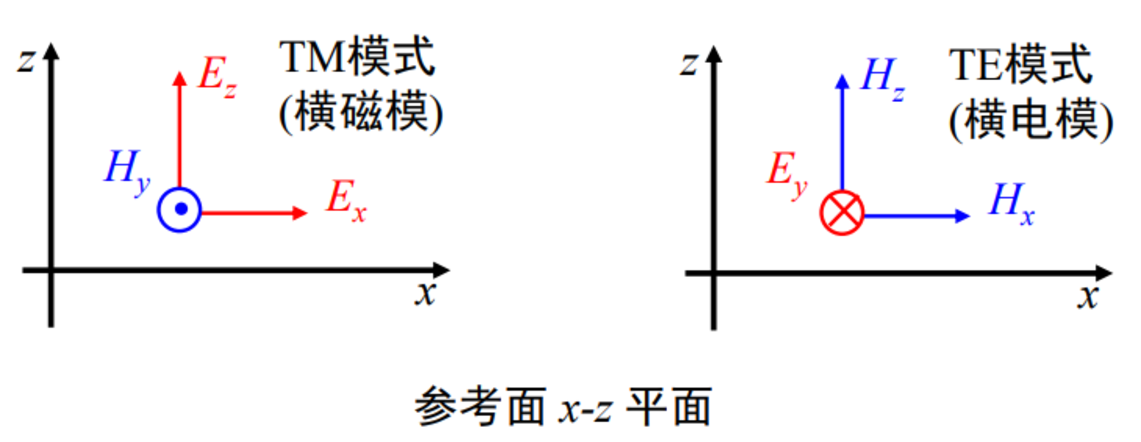
\includegraphics[width=0.7\textwidth]{L3/f2.pdf}
\caption{\justifying{两套独立解分别代表着TM模和TE模}}
\label{f3}
\end{figure}

\justifying{\setlength{\parindent}{2em}{考虑TE波的情况:由于在介质1和介质2的分界面有\fcolorbox{red}{white}{$H_x$和$E_y$切向连续}这一边界条件,故对\textcolor[rgb]{0,0,1}{$\pm k_zE_y=-i\omega\mu_0H_x$}运用边界条件,可得:}

\begin{align*}
\left\{
\begin{array}{l}  
  -k_{z1}E_{y1}=-i\omega\mu_0H_{x1} \text{(in Medium 1)}\vspace{1ex}\\
  k_{z2}E_{y2}=-i\omega\mu_0H_{x2} \text{(in Medium 2)}
\end{array} 
\right.
\end{align*}
两式相减,得到:
\[
E_y(k_{z1}+k_{z2})=0
\]
由于我们假设TE是以表面波的形式存在,故$k_{z1}$和$k_{z2}$都为正值,因此,为了使上式成立,只能使得$E_{y1}=E_{y2}=0$,显然,在TE波的假设下我们无法得到本征解,即SPP不可能是TE偏振。结合“思考题5”的情况,说明SPP只能是TM偏振。
\end{answer*}

\begin{problem} % 7
为什么SPP不能用空间光照射金属-介质界面直接激发?列举两种激发SPP的方法并说明其激发原理。
\end{problem}

\begin{answer*}

\justifying{\setlength{\parindent}{2em}{光波在传播的过程中严格满足动量守恒和能量守恒。其中,能量守恒保证了入射光和SPP的频率保持一致,动量守恒保证了入射光和SPP满足波矢匹配。而我们在“思考5”中已经得到SPP的色散关系:}
\[
\beta=k_0\sqrt{\dfrac{\varepsilon_1\varepsilon_2}{\varepsilon_1+\varepsilon_2}}=k_0\sqrt{\dfrac{\varepsilon_m\varepsilon_d}{\varepsilon_m+\varepsilon_d}}=k_0\sqrt{\dfrac{\varepsilon_d}{1-\dfrac{\varepsilon_d}{|\varepsilon_m|}}}=n_dk_0\sqrt{\dfrac{1}{1-\dfrac{\varepsilon_d}{|\varepsilon_m|}}}>n_dk_0
\]

这说明,SPP的传播常数比介质中的光波传播常数大,二者无法满足波矢匹配,即动量守恒,因此,SPP不能用空间光照射金属-介质界面直接激发。

\justifying{\setlength{\parindent}{2em}{常见的激发SPP的方法有棱镜耦合和高度集中光束激发。}

\fcolorbox{white}{green}{\mbox{1、棱镜耦合}}

\begin{figure}[H]
\centering
	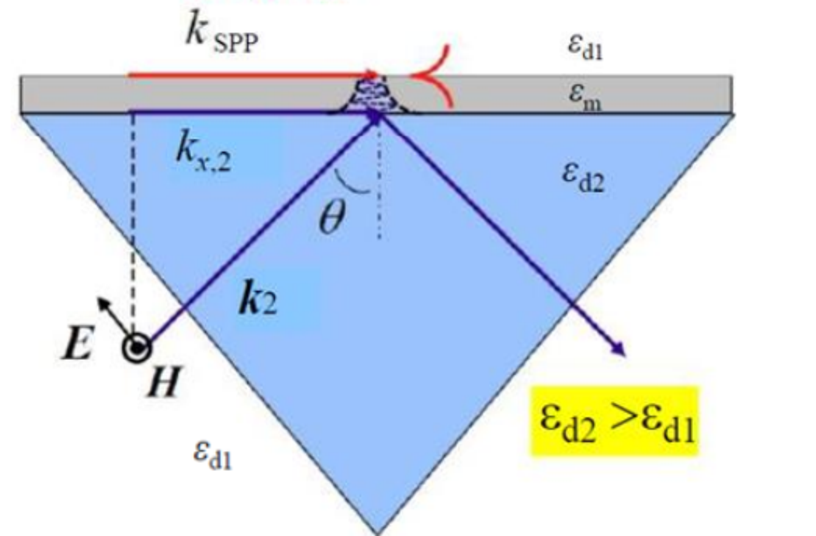
\includegraphics[width=0.4\textwidth]{L3/f3.pdf}
\caption{\justifying{棱镜耦合法示意图}}
\label{f4}
\end{figure}

\justifying{\setlength{\parindent}{2em}{原理:通过全内反射产生倏逝波(其传播常数为$\sqrt{\varepsilon_{d2}}k_0$),此时假设金属厚度$d$小于倏逝波的隧穿深度,那么当倏逝波发生隧穿透过金属薄膜达到介电常数小于棱镜的介质和金属表面时,其波矢与SPP的波矢一致,实现了动量守恒,这样就可以激发出SPP。此时,SPP传播常数为:}
\[
\beta=k_0\sqrt{\dfrac{\varepsilon_m\varepsilon_{d1}}{\varepsilon_m+\varepsilon_{d1}}}=\sqrt{\varepsilon_{d2}}k_0=k_{x2}
\]
入射角$\theta$需满足:
\[
\sin\theta=\sqrt{\dfrac{\varepsilon_m\varepsilon_{d1}}{(\varepsilon_m\varepsilon_{d1})\varepsilon_{d2}}}\qquad\&\qquad \theta>\theta_c
\]

\fcolorbox{white}{green}{\mbox{2、高度集中光束激发}}

\begin{figure}[H]
\centering
	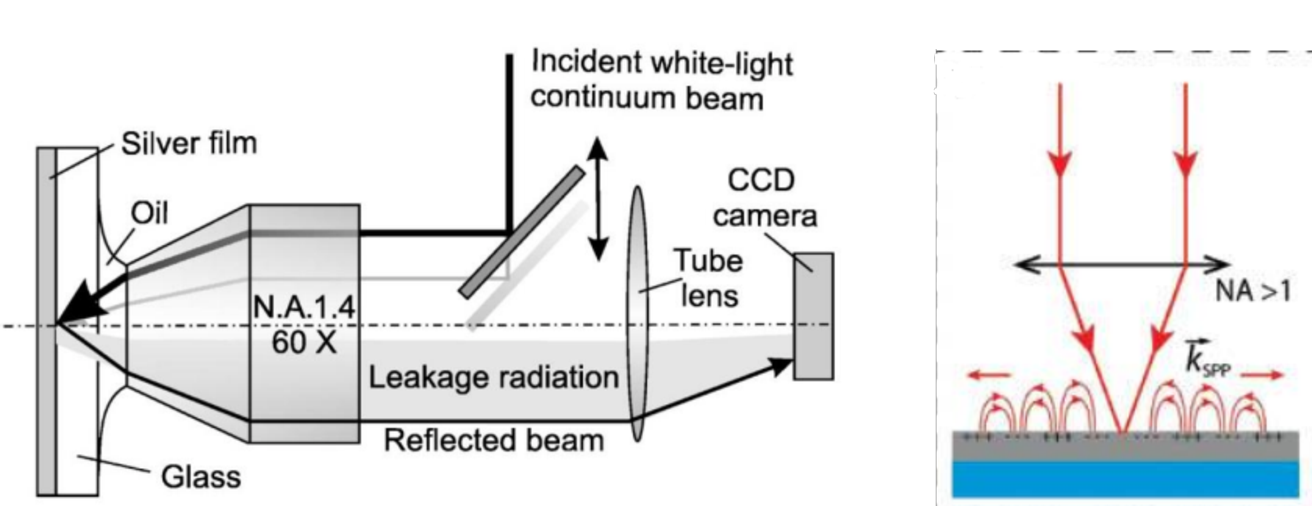
\includegraphics[width=0.7\textwidth]{L3/f4.pdf}
\caption{\justifying{高度集中光束激发法示意图}}
\label{f5}
\end{figure}

\justifying{\setlength{\parindent}{2em}{原理:利用具有高数值孔径的油浸物镜来代替棱镜,通过高度集中的光束来激发表面等离子体激元。由于其具有高的数值孔径,因而离轴光线的入射角很大,能保证全反射的发生,当$\theta>\theta_c$时,就可以激发SPP。}

\end{answer*}

\begin{problem} % 8
标准SPP的三个特征长度是什么,其物理意义是什么?
\end{problem}

\begin{answer*}

\justifying{\setlength{\parindent}{2em}{SPP的三个特征长度分别为:}

\justifying{\setlength{\parindent}{2em}{(1)金属中的衰减长度$\delta_m$,其物理意义是场穿透进金属中的深度,此时振荡强度减小为原来的1/e;}

\justifying{\setlength{\parindent}{2em}{(2)电介质中的衰减长度$\delta_d$,其物理意义是场穿透进介电材料中的深度,此时振荡强度减小为原来的1/e;}

\justifying{\setlength{\parindent}{2em}{(3)SPP的传播长度$\delta_{sp}$,其物理意义是沿$x$方向的场衰减为原来的1/e。由于这三个特征长度表征的均为强度的衰减,故它们的表达式中分母都有一个“2”。}
\begin{align*}
\left\{
\begin{array}{l}  
  \delta_m=\dfrac{1}{2k_{zm}}\vspace{1ex}\\
  \delta_d=\dfrac{1}{2k_{zd}}\vspace{1ex}\\
  \delta_{sp}=\dfrac{1}{2\beta''}
\end{array} 
\right.
\end{align*}

\justifying{\setlength{\parindent}{2em}{在集成光子学中,SPP的传播长度$\delta_{sp}$表征着光子回路的最大尺度;电介质中的衰减长度$\delta_d$表征着波长一半、元件的特征高度;金属中的衰减长度$\delta_m$表征着金属结构的最小的特征高度。}
\end{answer*}

\begin{problem} % 9
金属纳米颗粒链中为什么纵模颗粒之间电场是增强的而横模不是?
\end{problem}

\begin{answer*}

\begin{figure}[H]
\centering
	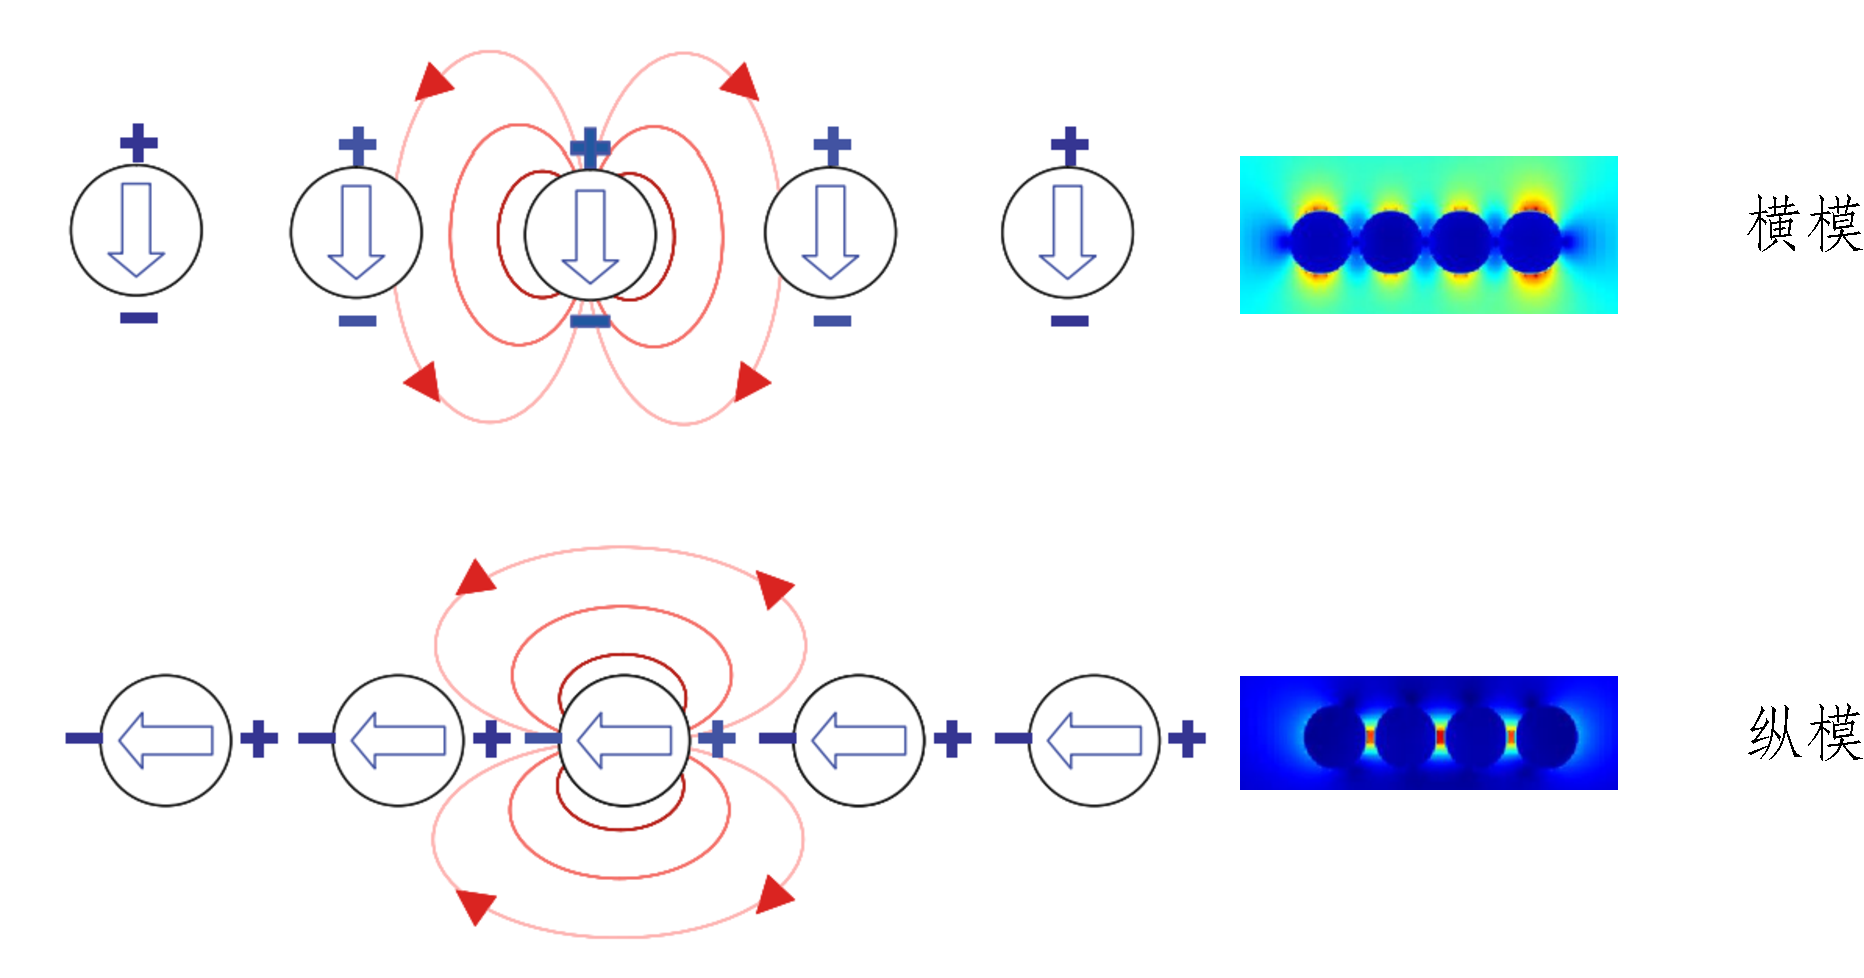
\includegraphics[width=0.7\textwidth]{L3/f6.pdf}
\caption{\justifying{两种不同极化的金属纳米颗粒之间的近场耦合示意图}}
\label{f7}
\end{figure}

\justifying{\setlength{\parindent}{2em}{对于纵模而言,一个金属纳米颗粒的偶极子作用在另一个金属纳米颗粒上的近场指向相同的方向,而对于横模,一个粒子的偶极子作用在另一个纳米颗粒上的近场指向相反的方向。因此,如果两个金属纳米颗粒一起被激发,则局域等离子体的电场在纵模情况下偶极振荡沿长轴方向,回复力减小,缝隙中的近场会增强,而在横模情况下则会减弱。从下图也可以看出,纵模情况下纳米颗粒之间的极化更强。}
\begin{figure}[H]
\centering
	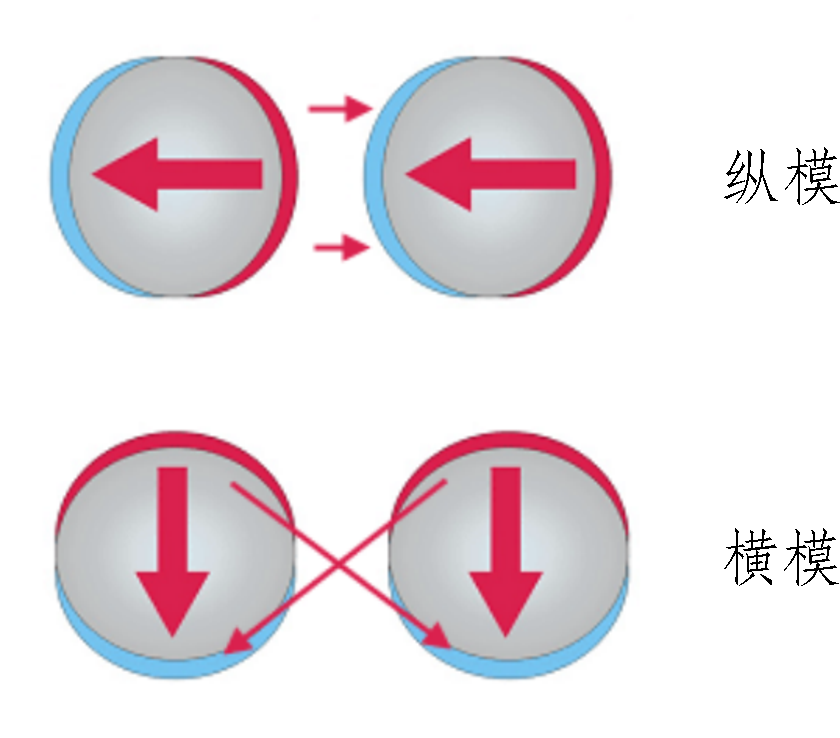
\includegraphics[width=0.3\textwidth]{L3/f7.pdf}
\caption{\justifying{关于激发光场的偏振,一对金属纳米颗粒的两种可能的情况。}}
\label{f8}
\end{figure}
当然,由于横模使得回复力增大,因而共振频率增大,吸收峰(谐振峰)向高频(短波)方向移动,简称蓝移;而纵模使得回复力增小,因而共振频率减小,吸收峰(谐振峰)向低频(长波)方向移动,简称红移。
\end{answer*}

\begin{problem} % 10
对于金属条带SPP波导,哪种情况下对场的束缚大?
\end{problem}

\begin{answer*}

\justifying{\setlength{\parindent}{2em}{对于金属条带SPP波导而言,短程SPP(SRSPP)波导对场的束缚更大,其金属条很厚,但缺点是传输距离短。}

\begin{figure}[H]
\centering
	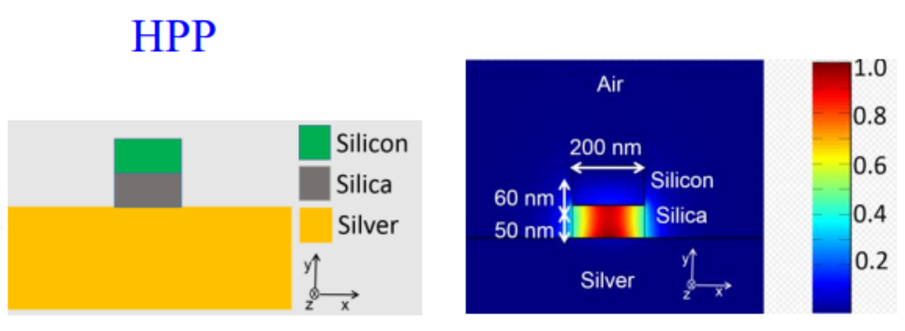
\includegraphics[width=0.6\textwidth]{L3/f8.pdf}
\caption{\justifying{混合SPP波导}}
\label{f9}
\end{figure}
\justifying{\setlength{\parindent}{2em}{混合波导结合了介质波导和金属波导的优点,可以实现低损耗、强约束,其SPP被很好地束缚在了金属和高折射率介质之间(在下图中则是被束缚在了二氧化硅中),且混合波导的传播长度可以到cm级。这种波导比前者对场的束缚更大。}
\end{answer*}

\begin{problem} % 11
如何得到LSP共振的Fr$\"{o}$hlish条件?
\end{problem}

\begin{answer*}

\justifying{\setlength{\parindent}{2em}{对于尺寸足够小($d\ll\lambda$)的纳米球而言,当把它放入均匀静电场中时,我们可以将其看做电偶极子,对其进行准静态近似,认为在同一时刻该粒子的不同位置的相位几乎相同。假设入射的均匀静电场表达式为$E_{\text{inc}}=E_0\boldsymbol{z}$,由于电势满足Laplace方程$\nabla^2\Phi=0$,故在准静态情况下可以利用$E=-\nabla\Phi$得到球内电场($E_{\text{in}}$)和球外电场($E_{\text{out}}$)。}

\begin{figure}[H]
\centering
	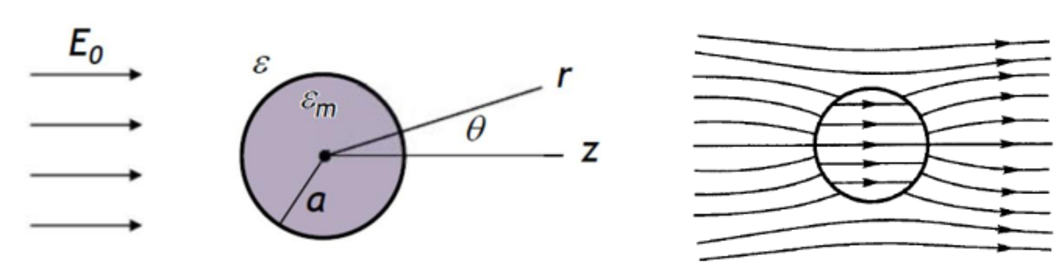
\includegraphics[width=0.7\textwidth]{L3/f5.pdf}
\caption{\justifying{位于静电场中的纳米微粒}}
\label{f6}
\end{figure}

\justifying{\setlength{\parindent}{2em}{使用以下边界条件:}
\[
\Phi_{\text{in}}|_{r=a}=\Phi_{\text{out}}|_{r=a},\qquad\varepsilon_0\varepsilon_m\dfrac{\partial\Phi_{\text{in}}}{\partial r}|_{r=a}=\varepsilon_0\varepsilon\dfrac{\partial\Phi_{\text{out}}}{\partial r}|_{r=a},\qquad\lim_{r \to \infty}\Phi_{\text{out}}=-E_0z
\]
可以求得:
\[
\Phi_{\text{in}}=\textcolor[rgb]{1,0,0}{-E_0r\cos\theta}+\dfrac{\varepsilon_m-\varepsilon}{\varepsilon_m+2\varepsilon}\cdot E_0r\cos\theta=-\dfrac{3\varepsilon}{\varepsilon_m+2\varepsilon}E_0r\cos\theta
\]
故球内的电场为:
\[
\boldsymbol{E}_{\text{in}}=-\nabla\Phi_{\text{in}}=\dfrac{3\varepsilon}{\varepsilon_m+2\varepsilon}\boldsymbol{E}_0
\]
考虑到偶极子位于介电常数为$\varepsilon$的介质中,则球内的电位移为:
\[
\boldsymbol{D}=\varepsilon_0\varepsilon_m\boldsymbol{E}_{\text{in}}=\varepsilon_0\boldsymbol{E}_{\text{in}}+\textcolor[rgb]{1,0,0}{\boldsymbol{P}_\varepsilon}+\boldsymbol{P}=\varepsilon_0\varepsilon\boldsymbol{E}_{\text{in}}+\boldsymbol{P}
\]
则偶极子对应的电极化强度为:
\[
\boldsymbol{P}=\varepsilon_0(\varepsilon_m-\varepsilon)\boldsymbol{E}=3\varepsilon_0\varepsilon\dfrac{\varepsilon_m-\varepsilon}{\varepsilon_m+2\varepsilon}\boldsymbol{E}_0
\]
整个球对应的电偶极矩为:
\[
\boldsymbol{p}=\boldsymbol{P}V=\dfrac{\varepsilon_m-\varepsilon}{\varepsilon_m+2\varepsilon}4\pi\varepsilon_0\varepsilon a^3\boldsymbol{E}_0
\]
由于极化率($\alpha$)定义为:
\[
\boldsymbol{p}=\varepsilon_0\varepsilon\textcolor[rgb]{1,0,0}{\alpha}\boldsymbol{E}_0
\]
因此,根据上面两式可以得到极化率为:
\[
\alpha=4\pi a^3\cdot\dfrac{\varepsilon_m-\varepsilon}{\varepsilon_m+2\varepsilon}
\]
其中$\varepsilon_m=\varepsilon_1(\omega)+i\varepsilon_2(\omega)$为金属的介电常数,而$\varepsilon$为背景介质的介电常数。

\justifying{\setlength{\parindent}{2em}{当发生共振现象的时候,这时电场能最强。故可以得到此时的谐振增强条件(Fr$\"{o}$hlish条件):}
\[
\textcolor[rgb]{1,0,0}{|\varepsilon_m(\omega)+2\varepsilon|=\text{minimum}}
\]
\end{answer*}












%\begin{problem}
%
%Consider the following decision rule for a two-category one-dimensional problem: 
%Decide \(\omega_1\) if \(x > \theta\); otherwise decide \(\omega_2\).
%
%(a) Show the probability of error for this rule is given by
%\[
%P(\text{error}) = P\left(\omega_{1}\right) \int_{-\infty}^{\theta} p\left(x | \omega_{1}\right) \mathrm{d}x+P\left(\omega_{2}\right) \int_{\theta}^{\infty} p\left(x | \omega_{2}\right) \mathrm{d}x.
%\]
%
%(b) By differentiating, show that a necessary condition to minimize \(P(\text{error})\) is that satisfy
%\[
%p(\theta | \omega_1) P(\omega_1) = p(\theta | \omega_2) P(\omega_2).
%\]
%
%(c) Does this equation define \(\theta\) uniquely?
%
%(d) Give an example where a value of \(\theta\) satisfying the equation actually maximizes the probability of error.
%
%\end{problem}
%
%\begin{answer}
%考虑分类错误率的条件概率:
%\begin{equation}
%	P(\text{error} | x) =
%	\begin{cases}
%		p(\omega_1 | x), & \text{if we decide }\omega_2, \\
%		p(\omega_2 | x), & \text{otherwise.}
%	\end{cases}
%	\label{eq:error-conditional-probability}
%\end{equation}
%
%根据式 (\ref{eq:error-conditional-probability}) 对\(x\)进行积分,可得:
%\begin{align}
%	P(\text{error}) & = \int_{-\infty}^\infty P(\text{error} | x) p(x) \mathrm{d} x \\
%	& = P(x \leq \theta , x \text{ is } \omega_1 ) + P(x > \theta , x \text{ is } \omega_2 ) \\
%	& = p(x \leq \theta | \omega_1) P(\omega_1) + p(x > \theta | \omega_2) P(\omega_2) \\
%	& = P\left(\omega_{1}\right) \int_{-\infty}^{\theta} p\left(x | \omega_{1}\right) \mathrm{d} x + P\left(\omega_{2}\right) \int_{\theta}^{\infty} p\left(x | \omega_{2}\right) \mathrm{d} x. \label{eq:error-probability}
%\end{align}
%\end{answer}
%
%\makecomputerexercise
%
%Several of the computer exercises will rely on the following data.
%
%此处还可以插入一些说明。
%
%\begin{computerexercise}
%Illustrate the fact that the average of a large number of independent random variables will approximate a Gaussian by the following:
%
%(a) Write a program to generate n random integers from a uniform distribution \(U(x_l, x_u)\).
%
%(b) Now write a routine to choose \(x_l\) and \(x_u\) randomly, in the range \(-100 \leq x_l < x_u \leq 100\), and \(n\) (the number of samples) randomly in the range \(0 < n \leq 1000\).
%
%(c) Generate and plot a histogram of the accumulation of \(10^4\) points sampled as just described.
%
%(d) Calculate the mean and standard deviation of your histogram, and plot it.
%
%(e) Repeat the above for \(10^5\) and for \(10^6\). Discuss your results.
%\end{computerexercise}
%
%\begin{answer}
%答案写在此处,如代码~\ref{lst:python}~所示。
%
%\begin{lstlisting}[language=python,caption=代码测试,label=lst:python]
%print('Hello, world!')
%\end{lstlisting}
%
%为了得到\(p(x | \omega) \sim \mathcal{N}(0, 1)\):
%\begin{equation}
%	p(x | \omega_i) = \frac{1}{\sqrt{2 \pi} \sigma}\exp{\left[- \frac{1}{2} \left(\frac{x - \mu}{\sigma}\right)^2\right]}
%	\label{eq:Gaussian-distribution}
%\end{equation}
%
%对式 (\ref{eq:Gaussian-distribution}),我们可以进行一些计算。
%
%\end{answer}
%
%%% 插入matlab代码
%\lstinputlisting[style=Matlab-editor,basicstyle=\mlttfamily,numbers=left,frame=single,caption={\bf main.m}]{L3/sample.m}
%%% 插入表格
%\begin{table}
%    \centering
%    \fontsize{8}{10}\selectfont    %{字体尺寸}{行距}
%    \caption{工作原理}
%	\begin{tblr}{
%        row{odd} = {bg=azure8},
%        row{1} = {bg=azure3, fg=white},
%        colspec={c|ccc},
%        }
%	    \toprule
%		\diagboxthree{偏振方向}{属性}{位置/晶向} & \mbox{左($\updownarrow$)} & \mbox{右($\odot$)} & \mbox{偏折} \\
%	    \specialrule{0.5pt}{4pt}{6pt}
%		$\updownarrow$ & \mbox{$e$($n$小)} & \mbox{$o$($n$大)} & \mbox{靠近法线}\\
%		$\odot$ & \mbox{$o$($n$大)} & \mbox{$e$($n$小)} & \mbox{远离法线}\\
%	    \bottomrule 
%	\end{tblr}
%    \label{tab:Training_sizes}
%\end{table}
%%% 插入图片
%\begin{figure}[H]
%\centering
%	\includegraphics[width=0.9\textwidth]{L3/Fig3_5.pdf}
%\caption{\justifying{Orientation of $\boldsymbol{E}$ vector at various locations along the $z$-axis.}}
%\label{f3_5}
%\end{figure}
%%% 首行缩进
%\justifying{\noindent 即此式也为直线方程,即出射光仍为线偏振光,只是振动面的方位较入射光即此式也为直线方程,即出射光仍为线偏振光,只是振动面的方位较入射光}
%
%\justifying{\setlength{\parindent}{2em} 即此式也为直线方程,即出射光仍为线偏振光,只是振动面的方位较入射光即此式也为直线方程,即出射光仍为线偏振光,只是振动面的方位较入射光}
%
%%% 引用参考文献
%\justifying{\noindent 显然,此式为直线方程,即线偏振光通过全波片后,其偏振状态不变。这里还有另一种理解方式\citep{ref3_1},现在,$\vv{a}$我们\fcolorbox{white}{green}{\mbox{我们}}考虑具有相同振幅的且具有相同相位(或相位差为$2\pi$整数倍)的两个波,在这里我们只考虑线偏振情况。}
%
%% 参考文献
%
%\begin{thebibliography}{23}
%
%\bibitem{ref3_1} %1
%Ashim Kumar Bain, ``Crystal Optics: Properties and Applications'', \sourcelink{10.1002/9783527823017}{Wiley Online} , Online ISBN: \textbf{9783527823017}(2019).
%
%\end{thebibliography}
\end{document}
